%% This is the main file and you use this file to organize your assignment.

\documentclass[a4paper]{article}	  
\usepackage[margin=3cm]{geometry} 	   % Choose your margin here. 
\usepackage{amsmath}
\usepackage{parskip}
\usepackage{graphicx}
\usepackage{caption}
\usepackage{subcaption}

\newcommand{\figref}[1]{\figurename~\ref{#1}}

\let\endtitlepage\relax						% Begin the text immidiately after the title page. Optional
\setlength{\parindent}{0cm}				% Start paragraph without indent. Optional

\begin{document}

\begin{titlepage}
\begin{center}
\Large TTK4190 Guidance and Control of Vehicles \\
\vspace{10pt}
\Large \LaTeX{} Template Assignment 1 \\
\vspace{10pt}
\large Written Fall 2019 By Name
\end{center}
\end{titlepage}

\section*{Info}
This is only a short template for the assignments and it is definitely not necessary to use this template if you are familiar with \LaTeX{} beforehand. The best way to learn \LaTeX{} is to write some stuff yourself and Google problems you run into. Therefore, we will not answer \LaTeX{} related questions outside of the assignment guidance, but you are of course welcome to ask questions then.

\section{Autopilot Design}
\subsection{}
The first order Nomoto model is a simple vessel model that we can use for this problem. The transfer function from rudder angle $\delta$ to heading rate $r = \dot \psi$ is given by equation (7.28) in \cite{Fossen2011} and is
\begin{equation}\begin{aligned}
\label{eq:nomoto_tf}
\frac{r}{\delta}(s) = \frac{K}{Ts + 1}
\end{aligned}\end{equation}
This corresponds to the time-domain representation
\begin{equation}\begin{aligned}
T \ddot \psi + \dot \psi = K \delta.
\end{aligned}\end{equation}

\subsection{}
In order to find the Nomoto parameters $T$ and $K$, we look at the step response of the system when excited by a reference $\delta_{\text{max}} = -25^{\circ}$, i.e. the maxiumum allowed rudder angle. Solving \eqref{eq:nomoto_tf} for the step response $r(t)$ we find
\begin{equation}\begin{aligned}
r(t) = \delta_{\text{max}} KT(1 - e^{-\frac{t}{T}}).
\end{aligned}\end{equation}
From classic control theory, we know that when $t = T$, $1 - e^{-\frac{t}{T}} = 1 - e^{-1} \approx 0.63$. In other words, the step response will hit $63\%$ of the final heading rate value $r_{\infty}$ at $t = T$. From \figref{fig:nomoto_reading} we see that this is at approximately $t = 140s$. Furthermore, as time goes to infinity, the exponential term goes to zero, and so $r$ approaches $\delta_{\text{max}} K T$. We read $r_\infty \approx 6.5 \cdot 10^{-3}$ from \figref{fig:nomoto_reading} and can then find $K$ as
\begin{equation}\begin{aligned}
K = \frac{r_{\infty}}{\delta_{\text{max}} T} \approx \frac{6.5 \cdot 10^{-3}}{25^{\circ} \cdot 140} \approx 1.06 \cdot 10^{-4}.
\end{aligned}\end{equation}
In total, we define the parameters
\begin{equation}\begin{aligned}
T = 140, \quad \text{and} \quad K = 1.06 \cdot 10^{-4}.
\end{aligned}\end{equation}

\begin{figure}[H]
\centering
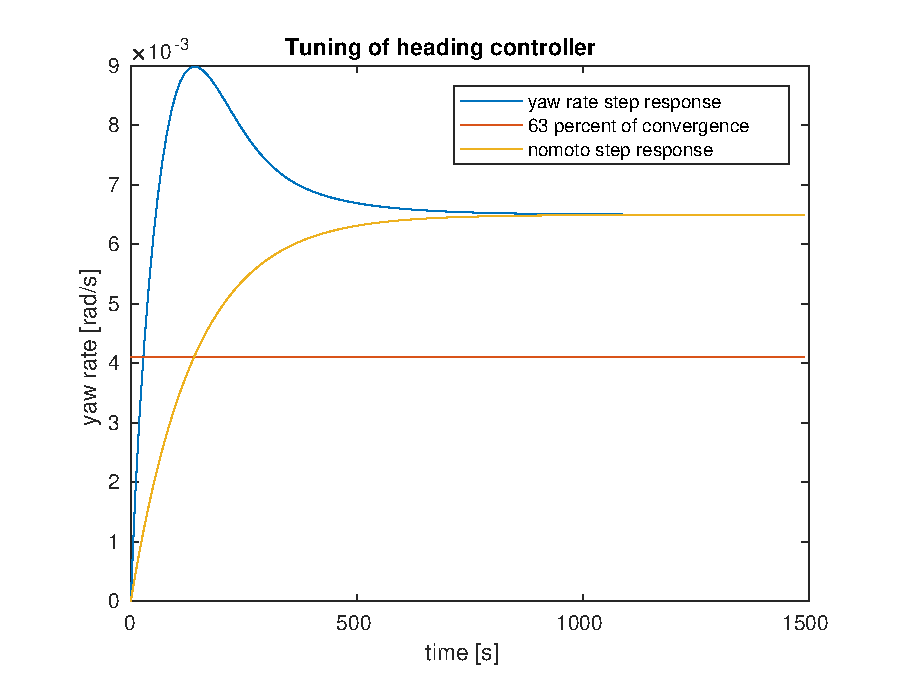
\includegraphics[width=0.7\textwidth]{nomoto-reading-improved}
\caption{Nomoto model parameter reading}
\label{fig:nomoto_reading}
\end{figure}


\subsection{}
We define a PD controller to control the heading $\psi$ from the rudder, i.e. we want the commanded rudder to be
\begin{equation}\begin{aligned}
\delta_c = -K_p (\psi_d - \psi) - K_d \psi_dot.
\end{aligned}\end{equation}
We wish to use the Nomoto model to find good values for $K_p$ and $K_d$. Using the model parameters, we define
\begin{equation}\begin{aligned}
T' = T \frac{U}{L_{pp}}, \quad K' = K \frac{L_{pp}}{U},
\end{aligned}\end{equation}
where $U = \sqrt{u^2 + v^2}$ is the ship velocity and $L_{pp}$ is the ship length. We also define
\begin{equation}\begin{aligned}
\omega_n = \sqrt{(\frac{u}{L_{pp}}) (\frac{1}{T})}, \quad \text{and} \quad \xi = 1.
\end{aligned}\end{equation}
With this, we choose the controller parameters
\begin{equation}\begin{aligned}
K_p = (\frac{L_{pp}}{U})^2 \frac{T'}{K'}, \quad \text{and} \quad
K_d = \frac{2 \xi \omega_n - 1}{K' \frac{U}{L_{pp}}}.
\end{aligned}\end{equation}
Since this control input will be input into a physical rudder, we have to saturate $\delta_c$ between the minimum and maximum rudder angles $-\delta_{\text{max}}$ and $\delta_{\text{max}}$. In addition, we could add rate limitation to the input, but we have not implemented this.



\begin{figure}[ht]
	\centering
	\begin{subfigure}[b]{0.45\textwidth}
		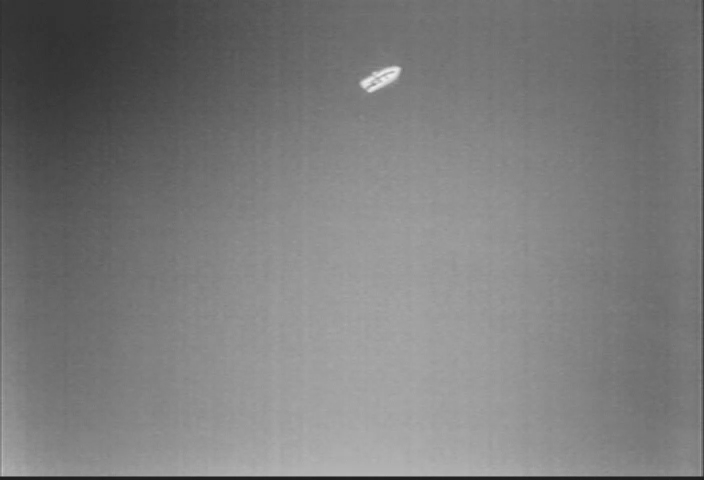
\includegraphics[width=\textwidth]{fig1}
		\caption{caption..}
		\label{fig:2a}
	\end{subfigure}
	~ %add desired spacing between images, e. g. ~, \quad, \qquad, \hfill etc.
	%(or a blank line to force the subfigure onto a new line)
	\begin{subfigure}[b]{0.45\textwidth}
		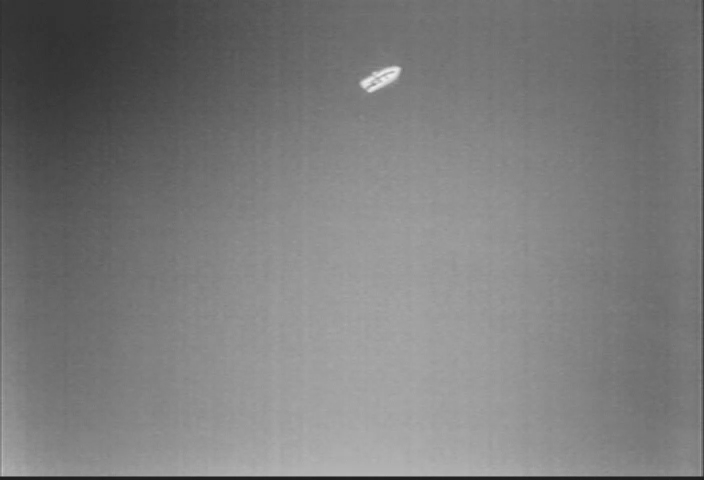
\includegraphics[width=\textwidth]{fig1}
		\caption{caption..}
		\label{fig:2b}
	\end{subfigure}
	\begin{subfigure}[b]{0.45\textwidth}
		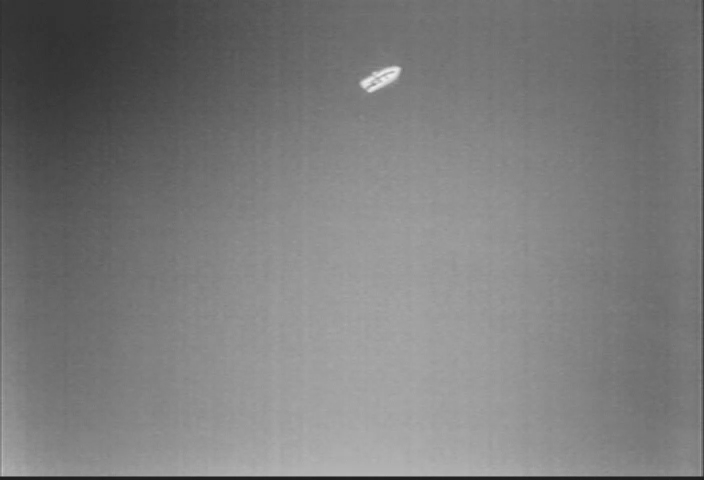
\includegraphics[width=\textwidth]{fig1}
		\caption{caption..}
		\label{fig:2c}
	\end{subfigure}
	\begin{subfigure}[b]{0.45\textwidth}
		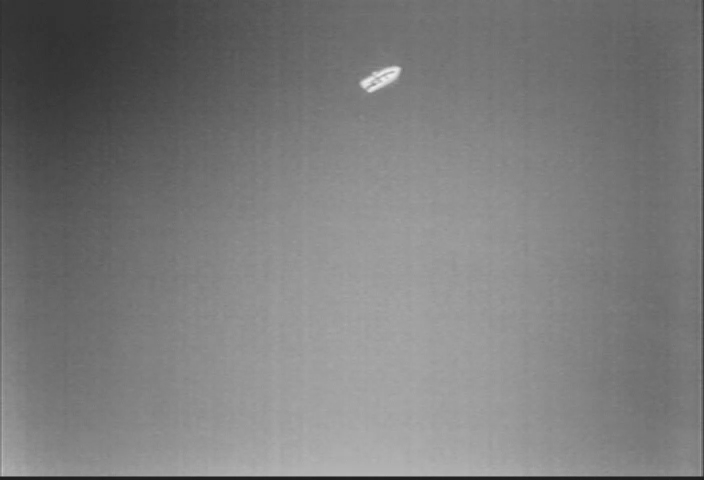
\includegraphics[width=\textwidth]{fig1}
		\caption{caption..}
		\label{fig:2d}
	\end{subfigure}
	\caption{Caption for all figures}\label{fig:2}
\end{figure}




	% Use "\include" instead of "\input" if you want the section to start on a new page. "problem1" is a tex file included at this location in the document. It is possible to answer the whole assignment in the main file (paste everything from "problem1.tex" and "problem2.tex" here), but that restricts the readability. Therefore, one file is created for each problem.
\section*{Problem 2 - Path Following with Crab angle Compensation}
\subsection*{Problem 2.1}
We implement a LOS guidance system using lookahead-based steering. The principle of this method is to move from one waypoint to the next by finding the LOS vector, and setting the desired course to move the vessel along this vector. Using the lookahead-based steering method, we separate the desired course a sum of the path-tangential angle and the velocity-path relative angle. The path-tangential angle can easily be found as the angle between the two waypoints, while the velocity-path relative angle can be found as using arctan of minus the cross-track error, divided by the distance between where the cross-track error and the LOS vector intercepts the line between the waypoints. 

We ended up choosing the same radius for all waypoints, set to be slightly larger than double the length of the vessel. Furthermore, we also limited delta to be between 0 and R. 

\subsection{Problem 2.2}
See \figref{fig:path_2_2} for the path of the vessel, and \figref{fig:cross_track_error2_2} for the cross-track error 

\begin{figure}[ht]
	\begin{subfigure}[b]{0.3\textwidth}
		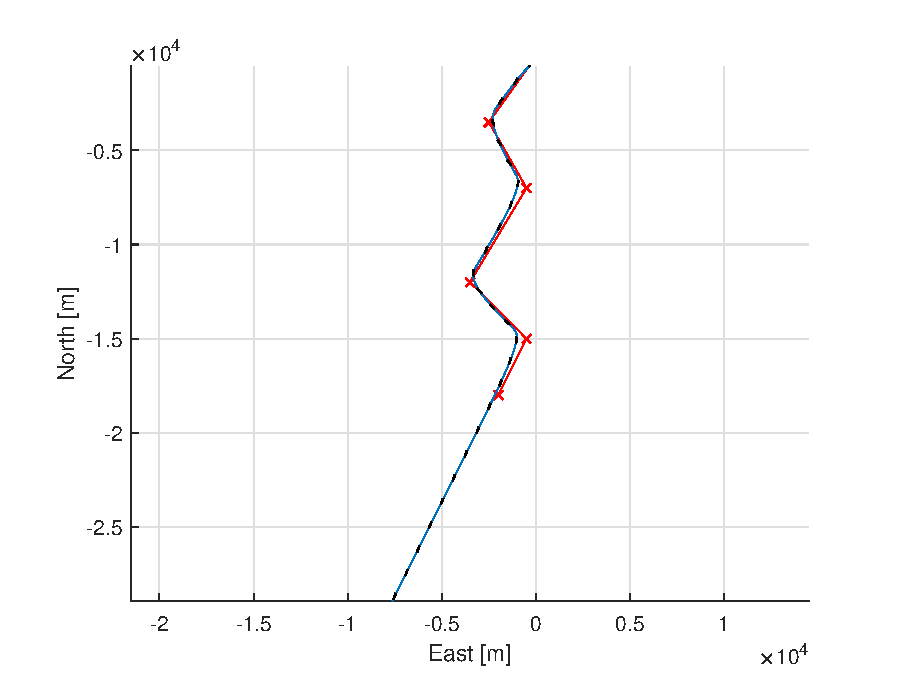
\includegraphics[width=\textwidth]{path_2_2}
		\caption{Path and waypoints}
		\label{fig:path_2_2}
	\end{subfigure}%
        ~
	\begin{subfigure}[b]{0.3\textwidth}
		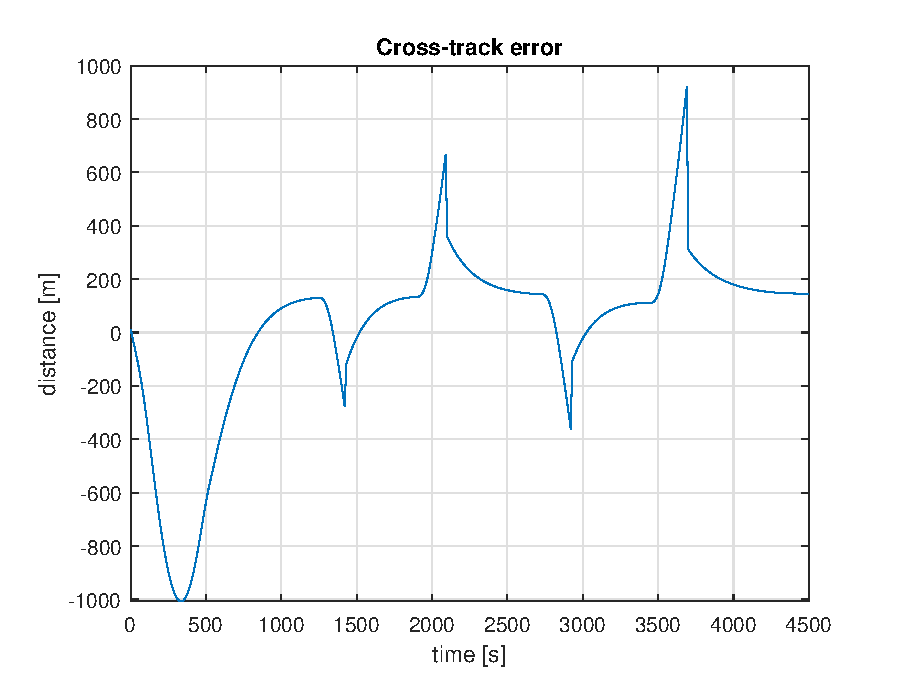
\includegraphics[width=\textwidth]{cross_track_error2_2}
		\caption{Rudder with saturation}
		\label{fig:cross_track_error2_2}
	\end{subfigure}
	\caption{Cross-track error}\label{fig:task2_2}
\end{figure}



Answer problem 2.1 here. The Greek letters for sideslip, heading and course are $\beta$, $\psi$ and $\chi$, respectively. Equation (10) in the assignment is:
\begin{equation}
\label{y_kinematics}
	\begin{aligned}
		\dot{x} &= u \cos (\psi) -v \sin (\psi) \\
		\dot{y} &= u \sin (\psi) + v \cos (\psi)
	\end{aligned}
\end{equation} 
You can refer to equations in the report by using the label and the "eqref" command. Example: equation \eqref{y_kinematics} shows the north and east velocities. 

\subsection*{Problem 2.2}
Answer Problem 2.2 here...

\subsection*{Problem 2.3}
Transfer functions can be written as
\begin{equation}
	H(s) = \frac{a_n s^n + ... + a_1 s + a_0}{b_m s^m + ... + b_1 s + b_0}
\end{equation}

The Nomoto model can be written as
\begin{equation}
\label{eq:nomoto}
	\begin{aligned}
		T \dot{r} + r &= K \delta + b \\
		\dot{\psi} &= r
	\end{aligned}
\end{equation}

\subsection*{Problem 2.4}
Answer Problem 2.4 here.  References can be placed in the "bibliography.bib" and referred to as \cite{Fossen2011} and \cite{Fjellstad1994857}. The PID-controller is
\begin{equation}
	\delta = -k_p y - k_d \dot{y} - k_i \int y
\end{equation}

 
\bibliographystyle{IEEEtran}
\bibliography{bibliography.bib}

\end{document}